%%%%%%%%%%%%%%%%%%%%%%%%%%%%%%%%%%%%%%%%%%%%%%%%%%%%%%%%%%%%%%%%%%%%%%%%%%
%%%%%%%%%%%%%%%%%%%%%%%%%%%%%%%%%%%%%%%%%%%%%%%%%%%%%%%%%%%%%%%%%%%%%%%%%%
\clearpage{}
\section{Measuring Anomalous Trilinear Gauge Couplings}
\label{sec:atgc}
% ---- ---- ---- ---- ---- ---- ---- ---- ---- ---- ---- ---- ---- ---- ----

The $s$-channel production of WW events occurs via the triple-gauge couplings 
WW$\gamma$ and WWZ.  
In the standard model, these couplings are defined  up to an overall constant. 
Contributions to these couplings from new physics processes would 
affect the measured WW cross section~\cite{Hagiwara1987253}.  
An effective Lagrangian can be used to describe the effect of non-SM 
processes on the $WWV$ couplings, where $V$ is either $\gamma$ or $\Z^0$. 
Such a Lagrangian contains a subset of the 14
possible terms consistent with Lorentz invariance~\cite{Hagiwara1987253}:
%%%%%%%%%%
\begin{equation*}
\frac{\mathcal{L}_{WWV}}{g_{WWV}}  = i g_1^V \left(
W^{\dagger}_{\mu\nu}W^{\mu}V^{\nu} -
W^{\dagger}_{\mu}V_{\nu}W^{\mu\nu} \right) + i\kappa_V
W^{\dagger}_{\mu}W_{\nu}V^{\mu\nu} + \frac{i\lambda}{M_W^2}
W^{\dagger}_{\lambda\mu} W^{\mu}_{\nu} V^{\nu\lambda} %% +
%% \frac{i\tilde{\lambda}}{M_W^2} W^{\dagger}_{\lambda\mu} W^{\mu}_{\
%% \nu} \hat{V}^{\nu\lambda},
\end{equation*}
%%%%%%%%%%%%%
\noindent
where $g_{WW\gamma} = -e,~g_{WWZ} = -e\cot\theta_W,~V_{\mu\nu} = \partial_{\mu} 
V_{\nu} - \partial_{\nu} V_{\mu}$, and $W_{\mu\nu} = \partial_{\mu} W_{\nu} - 
\partial_{\nu} W_{\mu}$.  
Demanding that the couplings are invariant
under $\mathrm{SU}(2)_L \times \mathrm{U}(1)_Y$ reduces the number
of coupling constants from 14 to 5 \cite{PhysRevD.41.2113}: 
$\lambda_Z$, $\Delta{\kappa_\gamma}$, $\Delta{g_1^Z}$, 
$\lambda_\gamma$ and $\Delta{\kappa_Z}$~\cite{MCFM}.
In the SM, $\kappa = 1$, and $\lambda = \tilde{\lambda} = 0$.
Assuming that the
coupling constants to $\gamma$ and $Z$ are the same 
further reduces the number to 3: 
$\lambda_Z$, $\Delta{\kappa_\gamma}$, and $\Delta{g_1^Z}$. 
The other two parameters ($\lambda_\gamma$ and $\Delta{\kappa_Z}$) 
can be written as functions of these three.
While we might want to search for anomalous couplings that differ for
$\gamma$ and $Z$, or are not invariant under the SM gauge symmetry,
the first search should be done in this restricted regime.  All
previous searches at hadron colliders have been done under these
assumptions.
In the present analysis, we additionally set $\Delta{g_1^Z} = 0$
(\textit{i.e.}, SM) and set limits on $\lambda_Z$ and $\Delta{\kappa_\gamma}$.


Individually, non-zero couplings lead to divergent WW cross 
section at high $\sqrt{s}$, and non-SM values of the $g_1^V$ or $\kappa_V$ 
couplings break the gauge cancellation of processes at high momentum transfer.  
However, there is no unique prescription to regulate this behavior or  
to apply a suppression factor, because such a regularization 
would depend on the scale of new physics which is unknown \textit{a priori}. 
{ \bf Hence, in the present analysis we do not apply any 
form factors or cut-off scale for new physics.}

%\cite{previous_searches}

%%We use the {\sc MCFM} program \cite{MCFM} to simulate the effects of
%%anomalous couplings as it is an accepted standard with calculations to
%%NLO.  Unfortunately, the output of MCFM is in a non-standard format
%%not easily interfaced to the CMS simulation framework.  Therefore, we
%%use the output of MCFM to understand the effects of anomalous
%%couplings on event variables and reweight standard CMS MC events to
%%match the MCFM distributions.
%%%%%%%%%%%%%%%%%%%%%%%%%%%%
%%%%%%%%%%%%%%%%%%%%%%%%%%%%
%%%%%%%%%%%%%%%%%%%%%%%%%%%%
\subsection{Existing limits}
The current best fit results for anomalous couplings are dominated by LEP results. 
Table~\ref{tab:aTGC_limits_fromPDG} shows the
existing limits for various couplings~\cite{PhysRevD.80.053012,pdg}.
Recent LHC measurements in the fully-leptonic final state 
(WW $\to\ell^+\nu\ell^-\overline{\nu}$) are approaching similar 
sensitivity~\cite{Chatrchyan:2011tz,Aad:2012ks}.
%%%%%%%%%%%%%%%%%%%%%%%%%%%%%
\begin{table}[h]
\caption{\label{tab:aTGC_limits_fromPDG}
Current limits on anomalous couplings. The world best limits are based on a fit of LEP
measurements. The LHC and Tevatron results are shown for comparison.}
\begin{center}
  \begin{tabular}{l c}
    \hline  \hline
   Coupling  &  Particle Data Group Fit\\\hline
   $\lambda_\gamma$  &  $0.028^{+0.020}_{- 0.021}$ \\
   $\lambda_Z$  &  $0.088^{+0.060}_{- 0.057}$ \\
   $\Delta{g_1^Z}$  &  $0.016^{+0.022}_{- 0.019}$ \\
   $\Delta{\kappa_\gamma}$  &  $0.027^{+0.044}_{- 0.045}$ \\
   $\Delta{\kappa_Z}$  &  $0.026^{+0.059}_{- 0.056}$ \\
    \hline  
\end{tabular}
\vskip 2mm
%%%%%%
  \begin{tabular}{l c c}
   \hline  
Coupling & Tevatron (WW +WZ $\to\ell\nu$2jet) & Tevatron (WW $\to\ell^+\nu\ell^-\overline{\nu}$)\\\hline
$\lambda = \lambda_\gamma = \lambda_Z$ & [-0.10,0.11] at 95\% C.L. & [-0.14,0.18] at 95\% C.L. \\
$\Delta{\kappa_\gamma}$  & [-0.44,0.55] at 95\% C.L. & [-0.54,0.83] at 95\% C.L. \\ 
$\Delta{g_1^Z}$  &   [-0.12,0.20] at 95\% C.L. & [-0.14,0.30] at 95\% C.L.\\
   \hline 
\end{tabular}
\vskip 2mm
%%%%%%
  \begin{tabular}{l c c}
   \hline  
Coupling & CMS 35~pb${}^{-1}$ (WW $\to\ell^+\nu\ell^-\overline{\nu}$) & ATLAS 1~fb${}^{-1}$ (WW $\to\ell^+\nu\ell^-\overline{\nu}$)\\\hline
$\lambda_Z$ & [-0.19,0.19] at 95\% C.L. & [-0.079,0.77] at 95\% C.L. \\
$\Delta{\kappa_\gamma}$  & [-0.61,0.65] at 95\% C.L. & [-0.071,0.071] at 95\% C.L. \\ 
$\Delta{g_1^Z}$  &   [-0.29,0.31] at 95\% C.L. & [-0.052,0.082] at 95\% C.L.\\
   \hline  \hline
\end{tabular}
\end{center}
\end{table}
%%%%%%%%%%%%%%%%%%%%%%%%%%%%%
%%%%%%%%%%%%%%%%%%%%%%%%%%%%
%%%%%%%%%%%%%%%%%%%%%%%%%%%%
%%%%%%%%%%%%%%%%%%%%%%%%%%%%
\subsection{Monte Carlo modeling of anomalous couplings}
We use the MCFM v6.0 NLO~\cite{MCFM} event generator to produce samples of 
1 million WW  events with and without anomalous couplings. 
The kinematic threshold values used to generate these events are  
summarized in Table~\ref{tab:MCFMSELECTION}.

%%%%%%%%%%%%%%%%%
\\
\begin{table}
\begin{center}
\caption{Kinematic threshold values used to generate events with and without anomalous couplings in MCFM.
\label{tab:MCFMSELECTION}}
\begin{tabular}{l l}
\hline \hline
         \Wln\ selection  & Jet selection \\ \hline 
          Lepton $p_{T} > 25~\GeV, |\eta| <2.5 $ & anti-$k_T$ 0.5, $p_{T}^{\textrm{jet}}> 30~\GeV, |\eta| <2.4$\\
          W transverse mass $> 50$~GeV     &  $\Delta \eta_{jj} < 1.5$ \\
          $\MET> 25$~GeV  & $\Delta \phi (\MET,\textrm{lead~jet}) > 0.4$  \\
\hline \hline
\end{tabular}
\end{center}
\end{table}
%%%%%%%%%%%%%%%%%
%%%%%%%%%%%%%%%%%%%%%%%%%%%%
\begin{figure}[h!t]
  {\centering
    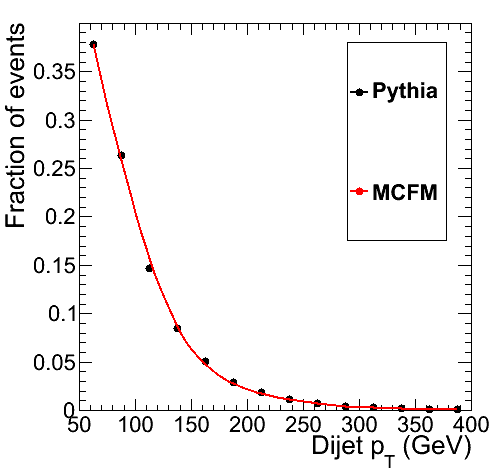
\includegraphics[width=0.48\textwidth]{figs/Pythia_mcfm_dijetpt.png}
    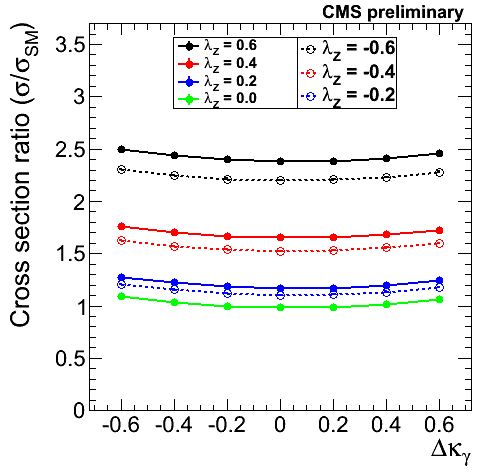
\includegraphics[width=0.48\textwidth]{figs/atgc_xsec2.png}
    \caption{(left) Comparison of the dijet $p_T$ distribution for WW events in Pythia 
    (after Gen--RECO matching) and LO MCFM. The agreement between the two is good.
    (right) Change in cross section relative to the standard model couplings 
    as a function of $\lambda_Z$ and $\Delta{\kappa_\gamma}$.
    }
    \label{fig:ww_dijetPt_PythiaMCFM_comparison}}
\end{figure}
%%%%%%%%%%%%%%%%%%%%%%%%%%%%
%%%%%%%%%%%%%%%%%%%%%%%%%%%%
%%%%%%%%%%%%%%%%%%%%%%%%%%%%
\begin{figure}[h!t]
  {\centering
    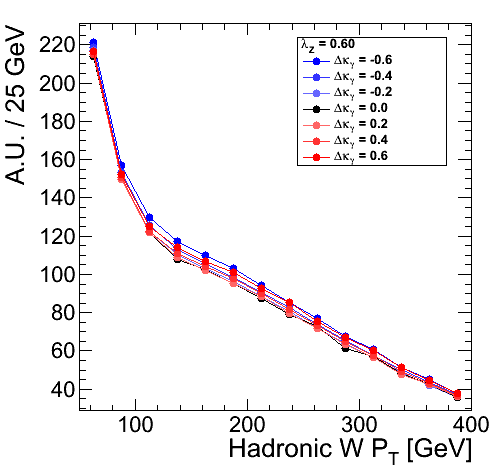
\includegraphics[width=0.48\textwidth]{figs/HadronicWpT_060.png}
    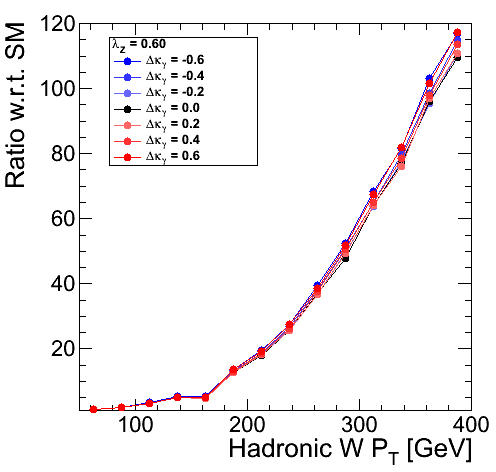
\includegraphics[width=0.48\textwidth]{figs/HadronicWpT_060_ratio.png}
    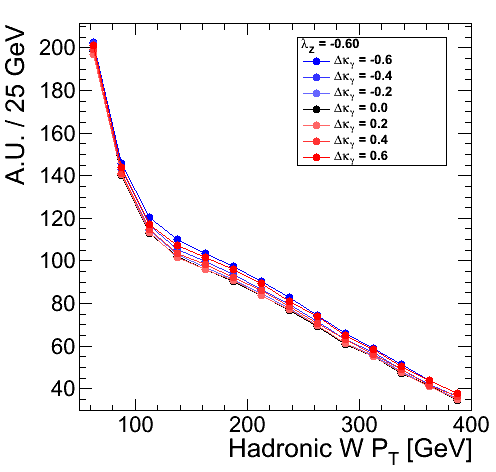
\includegraphics[width=0.48\textwidth]{figs/HadronicWpT_m060.png}
    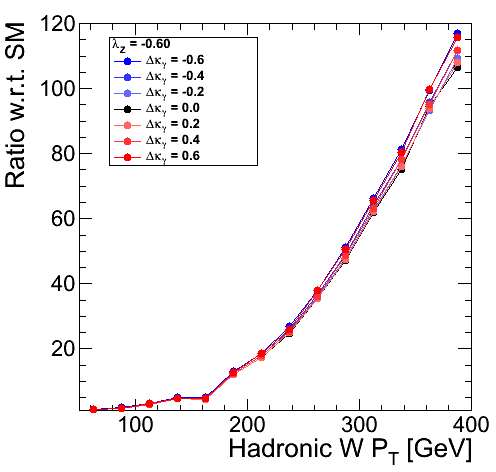
\includegraphics[width=0.48\textwidth]{figs/HadronicWpT_m060_ratio.png}
    \caption{Dijet $p_T$ distribution (left) and its ratio relative to 
    the standard model coupling (right) for $\lambda_Z = \pm 0.6$ and various choices of $\Delta{\kappa_\gamma}$.}
    \label{fig:ww_dijetPt_atgcRatio06}}
\end{figure}
%%%%%%%%%%%%%%%%%%%%%%%%%%%%
\begin{figure}[h!t]
  {\centering
    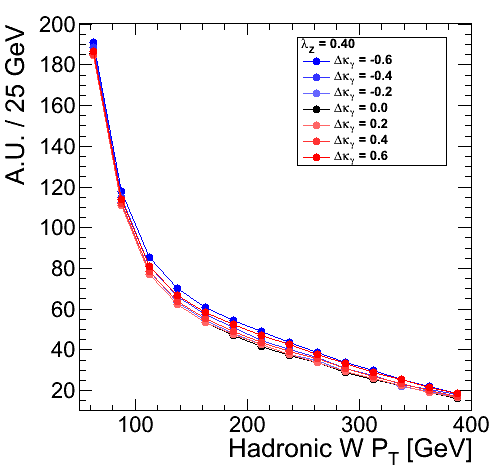
\includegraphics[width=0.48\textwidth]{figs/HadronicWpT_040.png}
    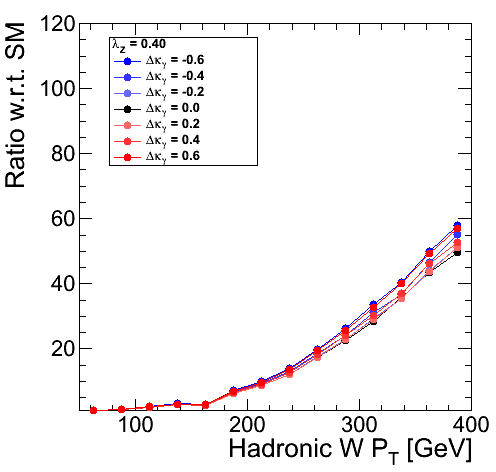
\includegraphics[width=0.48\textwidth]{figs/HadronicWpT_040_ratio.png}
    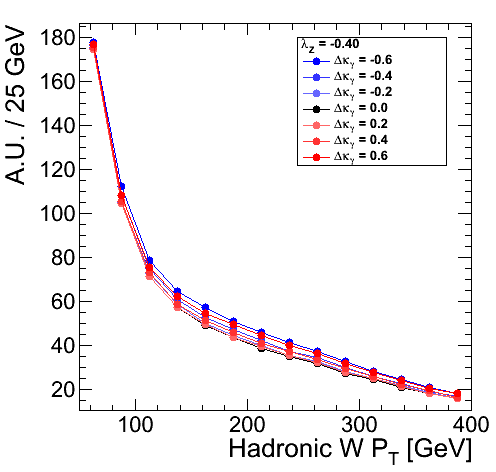
\includegraphics[width=0.48\textwidth]{figs/HadronicWpT_m040.png}
    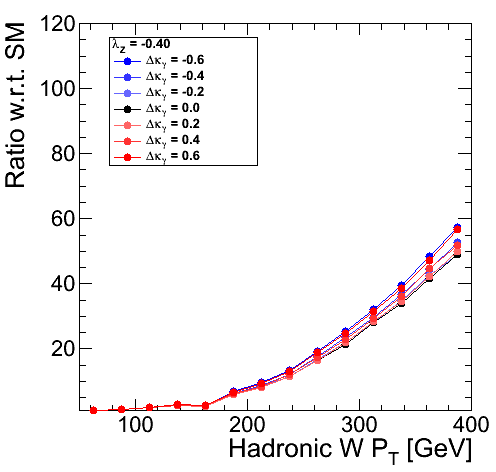
\includegraphics[width=0.48\textwidth]{figs/HadronicWpT_m040_ratio.png}
    \caption{Dijet $p_T$ distribution (left) and its ratio relative to 
    the standard model coupling (right) for $\lambda_Z = \pm 0.4$ and various choices of $\Delta{\kappa_\gamma}$.}
    \label{fig:ww_dijetPt_atgcRatio04}}
\end{figure}
%%%%%%%%%%%%%%%%%%%%%%%%%%%%
%%%%%%%%%%%%%%%%%%%%%%%%%%%%
\begin{figure}[h!t]
  {\centering
    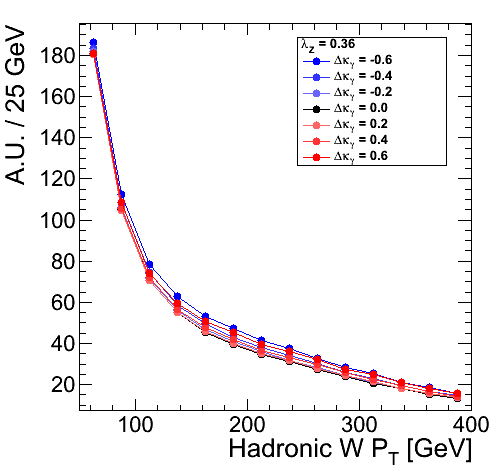
\includegraphics[width=0.48\textwidth]{figs/HadronicWpT_036.png}
    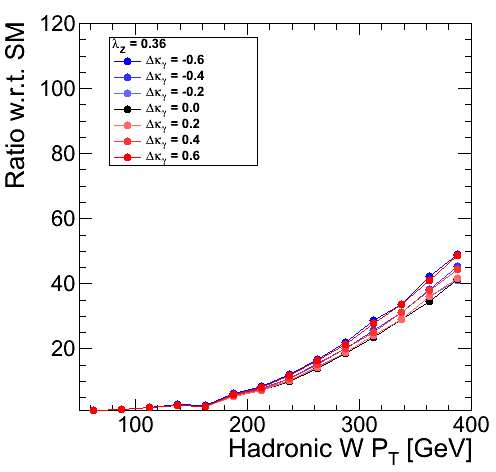
\includegraphics[width=0.48\textwidth]{figs/HadronicWpT_036_ratio.png}
    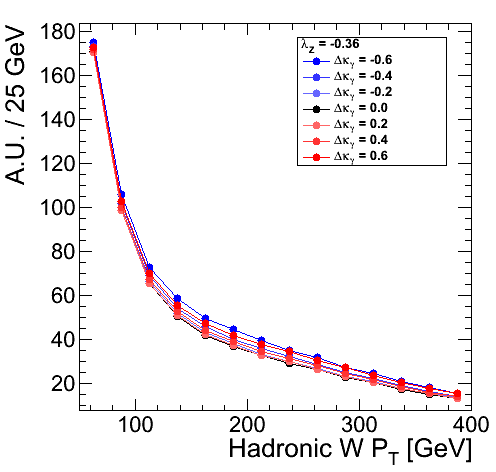
\includegraphics[width=0.48\textwidth]{figs/HadronicWpT_m036.png}
    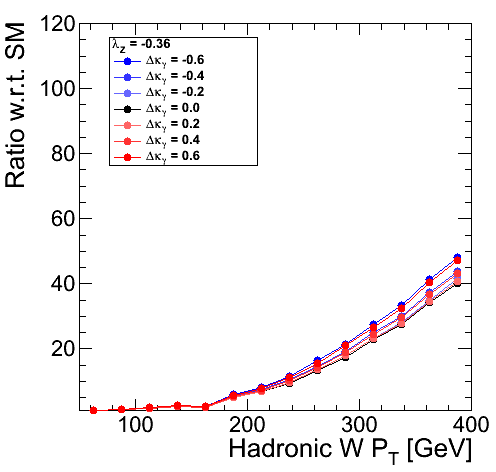
\includegraphics[width=0.48\textwidth]{figs/HadronicWpT_m036_ratio.png}
    \caption{Dijet $p_T$ distribution (left) and its ratio relative to 
    the standard model coupling (right) for $\lambda_Z = \pm 0.36$ and various choices of $\Delta{\kappa_\gamma}$.}
    \label{fig:ww_dijetPt_atgcRatio036}}
\end{figure}
%%%%%%%%%%%%%%%%%%%%%%%%%%%%
%%%%%%%%%%%%%%%%%%%%%%%%%%%%
\begin{figure}[h!t]
  {\centering
    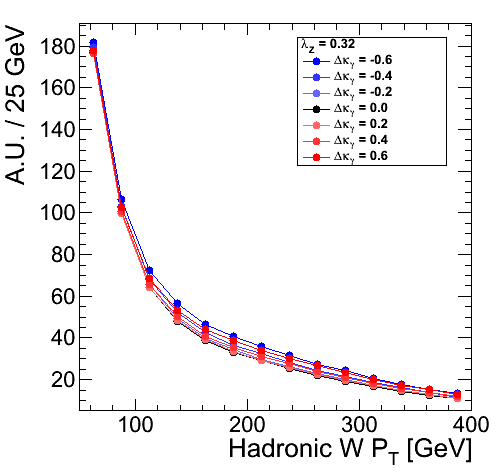
\includegraphics[width=0.48\textwidth]{figs/HadronicWpT_032.png}
    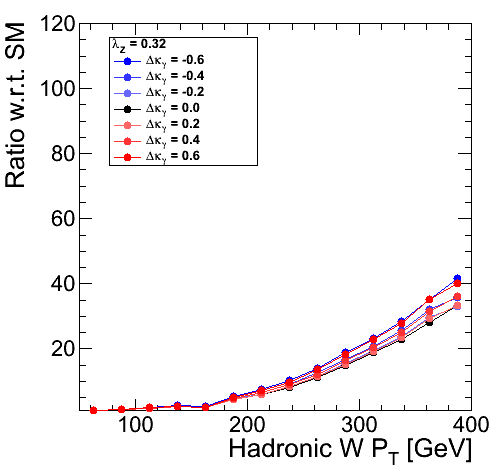
\includegraphics[width=0.48\textwidth]{figs/HadronicWpT_032_ratio.png}
    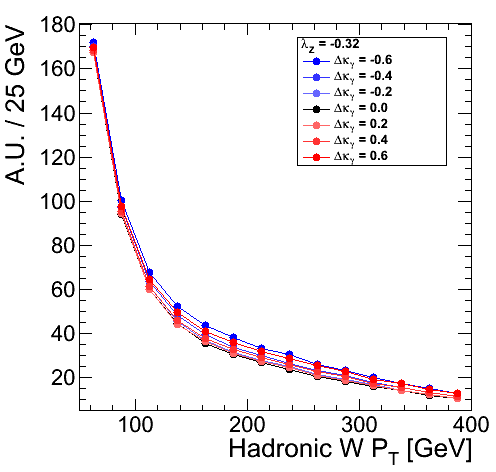
\includegraphics[width=0.48\textwidth]{figs/HadronicWpT_m032.png}
    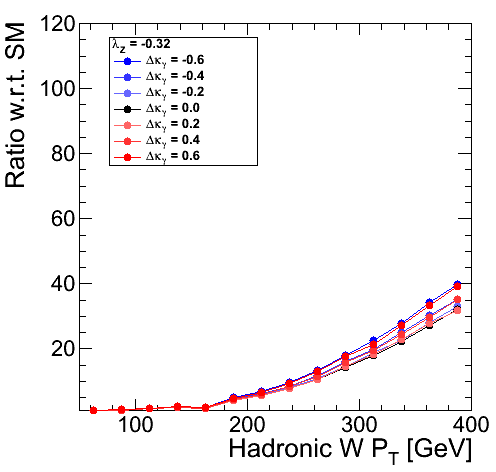
\includegraphics[width=0.48\textwidth]{figs/HadronicWpT_m032_ratio.png}
    \caption{Dijet $p_T$ distribution (left) and its ratio relative to 
    the standard model coupling (right) for $\lambda_Z = \pm 0.32$ and various choices of $\Delta{\kappa_\gamma}$.}
    \label{fig:ww_dijetPt_atgcRatio032}}
\end{figure}
%%%%%%%%%%%%%%%%%%%%%%%%%%%%
%%%%%%%%%%%%%%%%%%%%%%%%%%%%
\begin{figure}[h!t]
  {\centering
    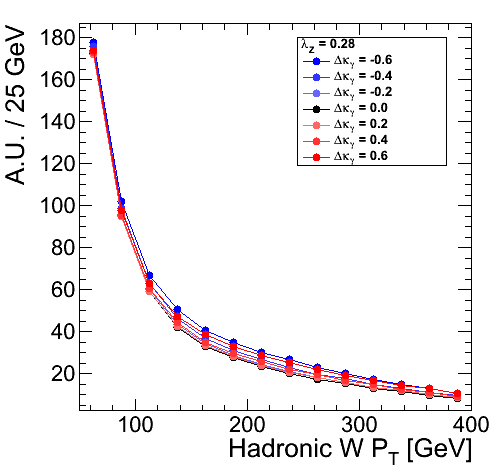
\includegraphics[width=0.48\textwidth]{figs/HadronicWpT_028.png}
    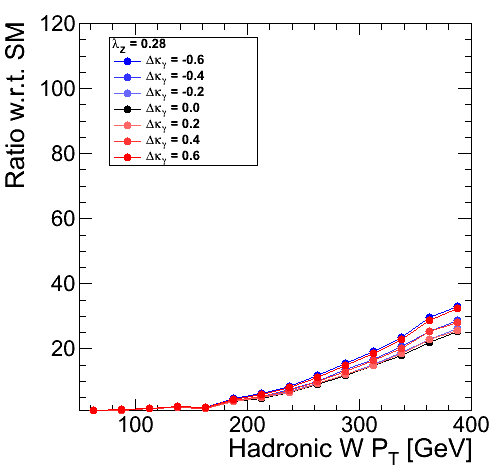
\includegraphics[width=0.48\textwidth]{figs/HadronicWpT_028_ratio.png}
    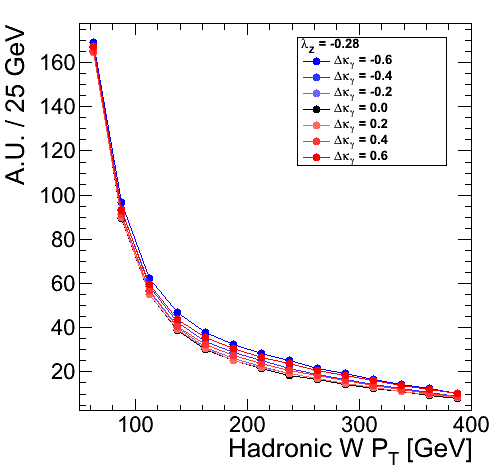
\includegraphics[width=0.48\textwidth]{figs/HadronicWpT_m028.png}
    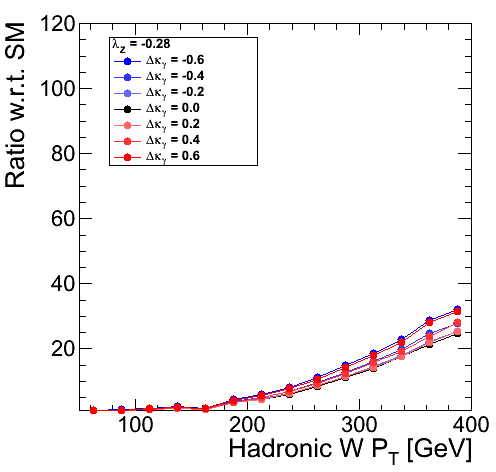
\includegraphics[width=0.48\textwidth]{figs/HadronicWpT_m028_ratio.png}
    \caption{Dijet $p_T$ distribution (left) and its ratio relative to 
    the standard model coupling (right) for $\lambda_Z = \pm 0.28$ and various choices of $\Delta{\kappa_\gamma}$.}
    \label{fig:ww_dijetPt_atgcRatio028}}
\end{figure}
%%%%%%%%%%%%%%%%%%%%%%%%%%%%
%%%%%%%%%%%%%%%%%%%%%%%%%%%%
\begin{figure}[h!t]
  {\centering
    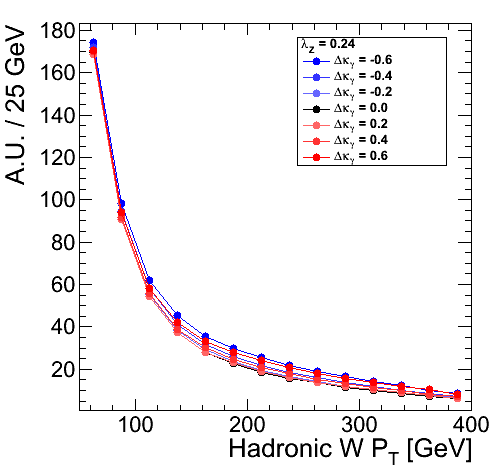
\includegraphics[width=0.48\textwidth]{figs/HadronicWpT_024.png}
    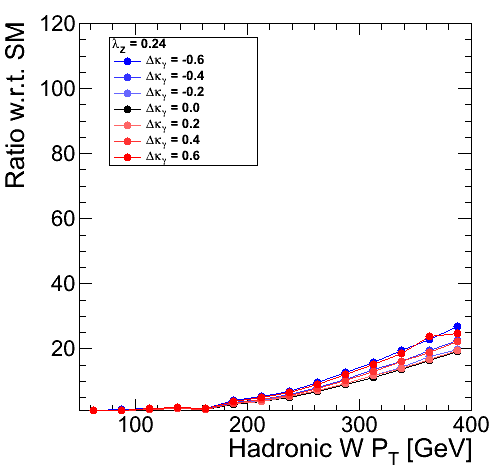
\includegraphics[width=0.48\textwidth]{figs/HadronicWpT_024_ratio.png}
    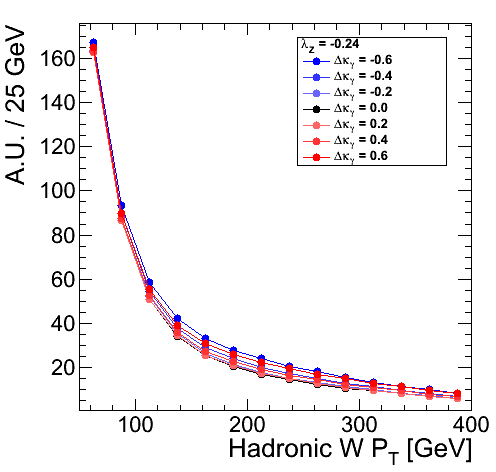
\includegraphics[width=0.48\textwidth]{figs/HadronicWpT_m024.png}
    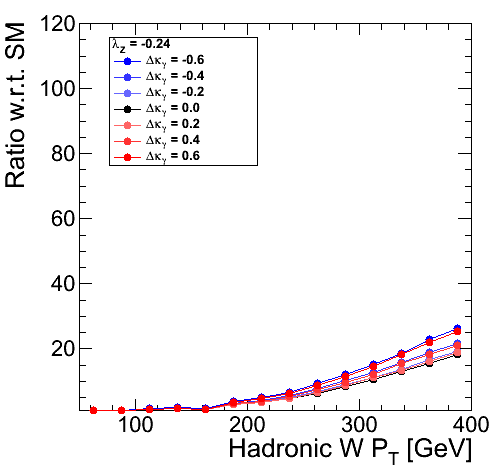
\includegraphics[width=0.48\textwidth]{figs/HadronicWpT_m024_ratio.png}
    \caption{Dijet $p_T$ distribution (left) and its ratio relative to 
    the standard model coupling (right) for $\lambda_Z = \pm 0.24$ and various choices of $\Delta{\kappa_\gamma}$.}
    \label{fig:ww_dijetPt_atgcRatio024}}
\end{figure}
%%%%%%%%%%%%%%%%%%%%%%%%%%%%
%%%%%%%%%%%%%%%%%%%%%%%%%%%%
\begin{figure}[h!t]
  {\centering
    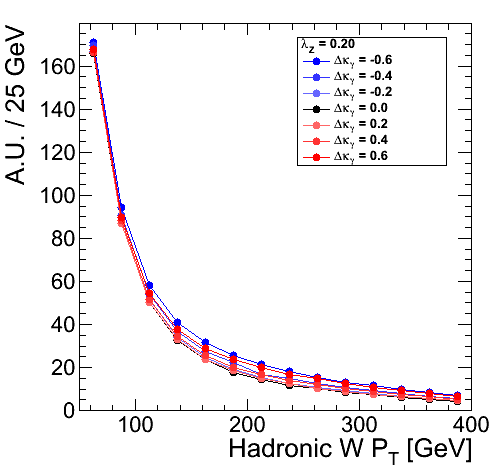
\includegraphics[width=0.48\textwidth]{figs/HadronicWpT_020.png}
    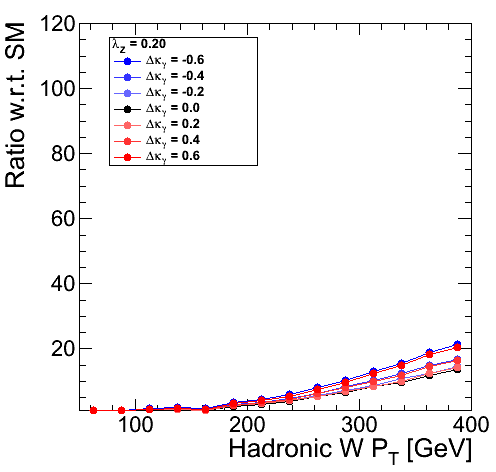
\includegraphics[width=0.48\textwidth]{figs/HadronicWpT_020_ratio.png}
    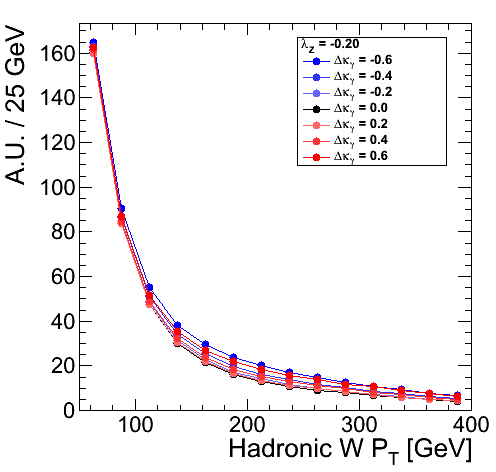
\includegraphics[width=0.48\textwidth]{figs/HadronicWpT_m020.png}
    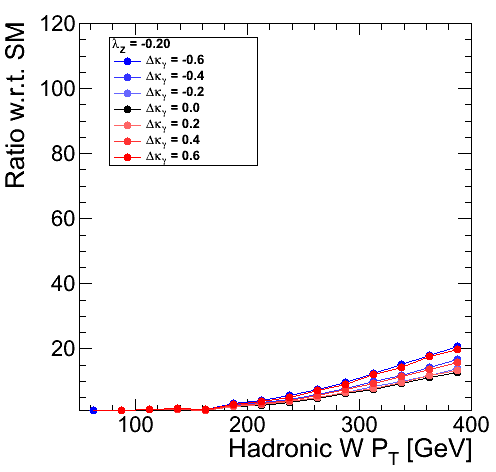
\includegraphics[width=0.48\textwidth]{figs/HadronicWpT_m020_ratio.png}
    \caption{Dijet $p_T$ distribution (left) and its ratio relative to 
    the standard model coupling (right) for $\lambda_Z = \pm 0.20$ and various choices of $\Delta{\kappa_\gamma}$.}
    \label{fig:ww_dijetPt_atgcRatio020}}
\end{figure}
%%%%%%%%%%%%%%%%%%%%%%%%%%%%
%%%%%%%%%%%%%%%%%%%%%%%%%%%%
\begin{figure}[h!t]
  {\centering
    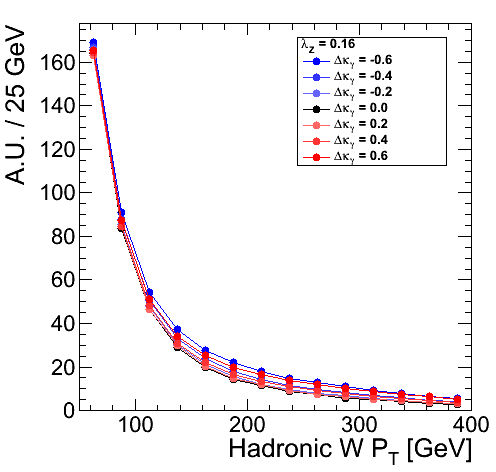
\includegraphics[width=0.48\textwidth]{figs/HadronicWpT_016.png}
    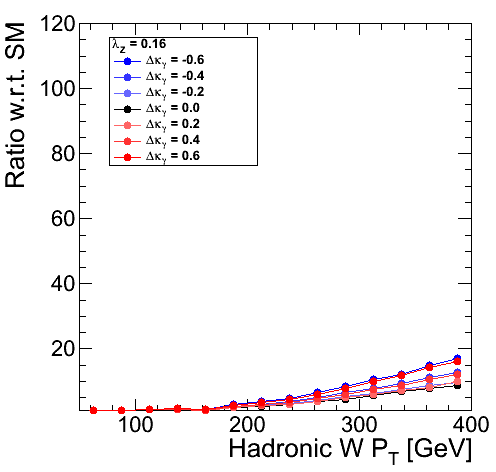
\includegraphics[width=0.48\textwidth]{figs/HadronicWpT_016_ratio.png}
    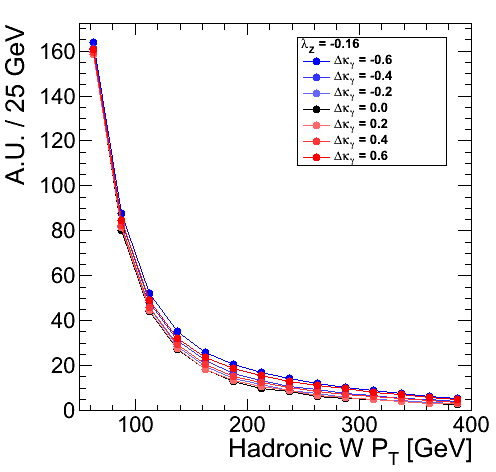
\includegraphics[width=0.48\textwidth]{figs/HadronicWpT_m016.png}
    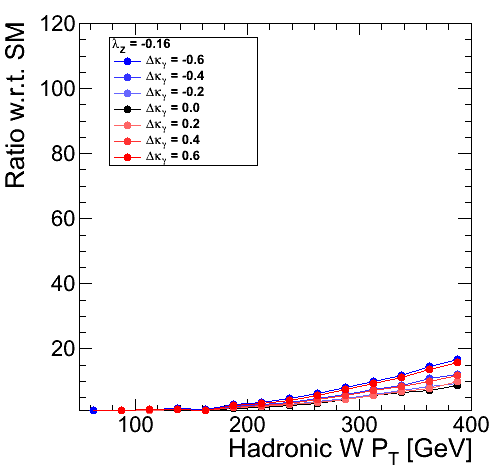
\includegraphics[width=0.48\textwidth]{figs/HadronicWpT_m016_ratio.png}
    \caption{Dijet $p_T$ distribution (left) and its ratio relative to 
    the standard model coupling (right) for $\lambda_Z = \pm 0.16$ and various choices of $\Delta{\kappa_\gamma}$.}
    \label{fig:ww_dijetPt_atgcRatio016}}
\end{figure}
%%%%%%%%%%%%%%%%%%%%%%%%%%%%
%%%%%%%%%%%%%%%%%%%%%%%%%%%%
\begin{figure}[h!t]
  {\centering
    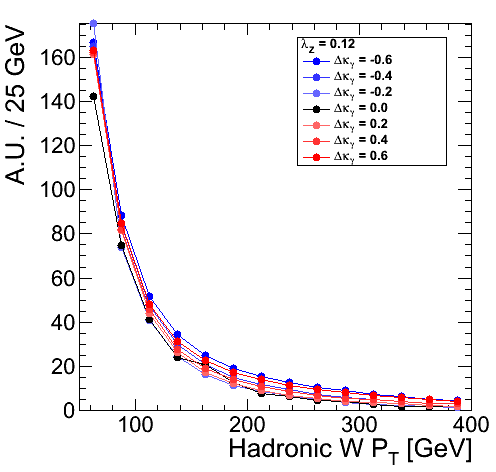
\includegraphics[width=0.48\textwidth]{figs/HadronicWpT_012.png}
    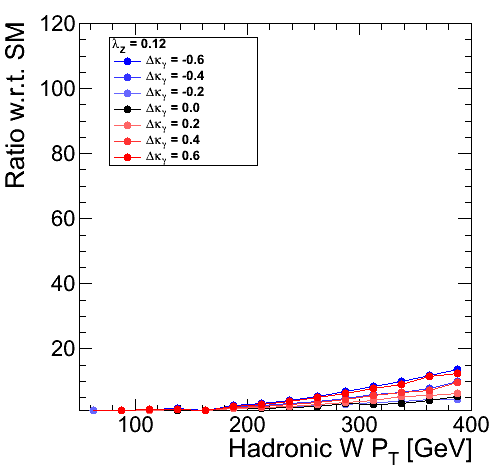
\includegraphics[width=0.48\textwidth]{figs/HadronicWpT_012_ratio.png}
    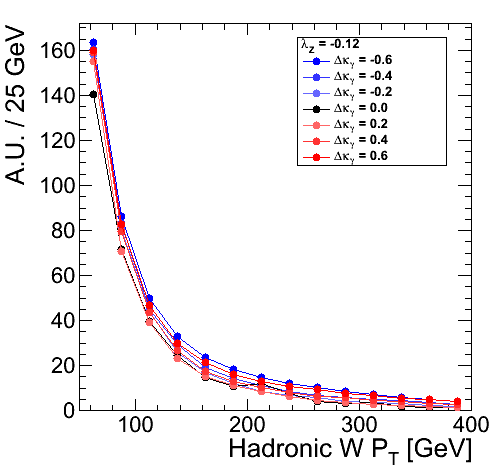
\includegraphics[width=0.48\textwidth]{figs/HadronicWpT_m012.png}
    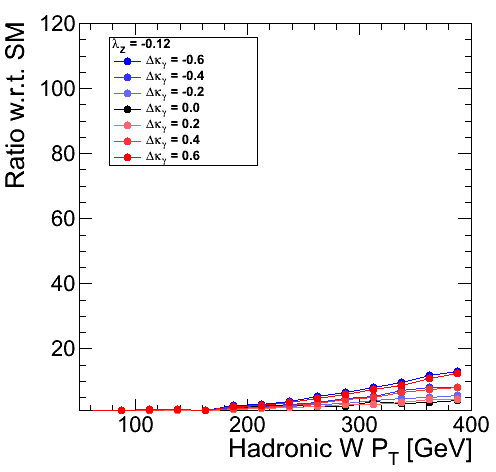
\includegraphics[width=0.48\textwidth]{figs/HadronicWpT_m012_ratio.png}
    \caption{Dijet $p_T$ distribution (left) and its ratio relative to 
    the standard model coupling (right) for $\lambda_Z = \pm 0.12$ and various choices of $\Delta{\kappa_\gamma}$.}
    \label{fig:ww_dijetPt_atgcRatio012}}
\end{figure}
%%%%%%%%%%%%%%%%%%%%%%%%%%%%
%%%%%%%%%%%%%%%%%%%%%%%%%%%%
\begin{figure}[h!t]
  {\centering
    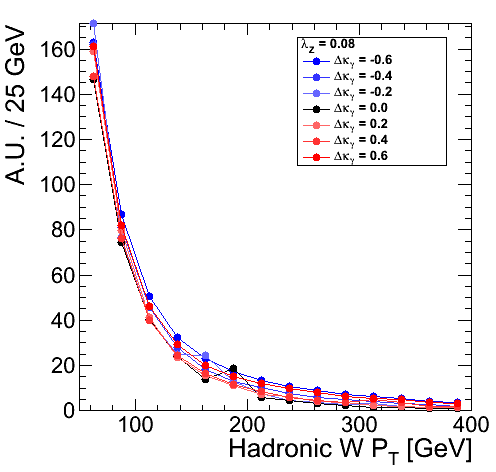
\includegraphics[width=0.48\textwidth]{figs/HadronicWpT_008.png}
    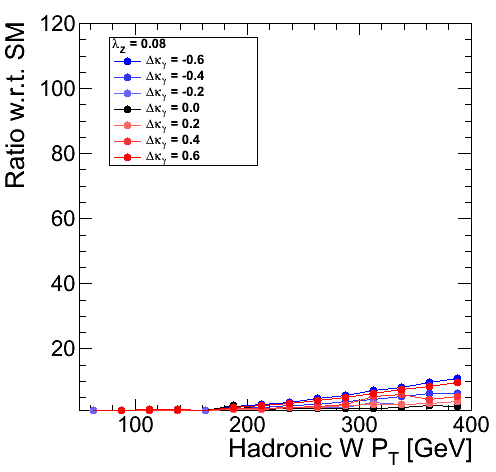
\includegraphics[width=0.48\textwidth]{figs/HadronicWpT_008_ratio.png}
    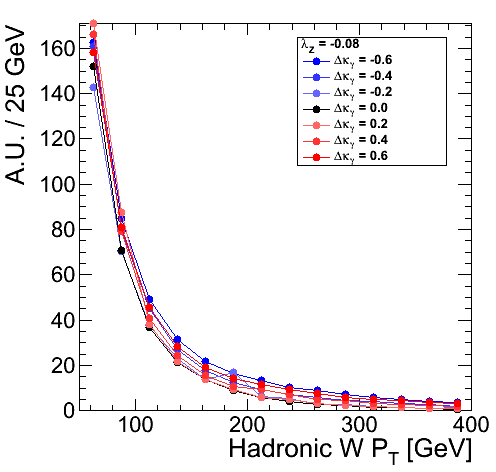
\includegraphics[width=0.48\textwidth]{figs/HadronicWpT_m008.png}
    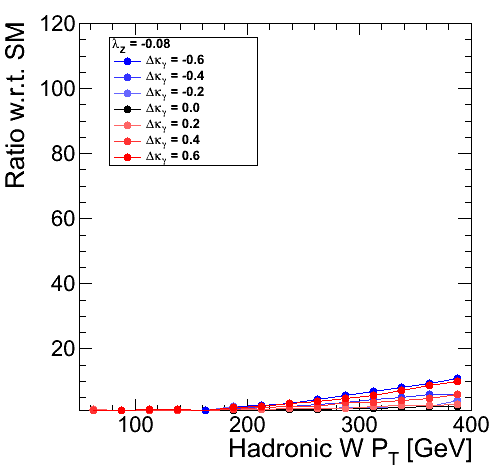
\includegraphics[width=0.48\textwidth]{figs/HadronicWpT_m008_ratio.png}
    \caption{Dijet $p_T$ distribution (left) and its ratio relative to 
    the standard model coupling (right) for $\lambda_Z = \pm 0.08$ and various choices of $\Delta{\kappa_\gamma}$.}
    \label{fig:ww_dijetPt_atgcRatio008}}
\end{figure}
%%%%%%%%%%%%%%%%%%%%%%%%%%%%
%%%%%%%%%%%%%%%%%%%%%%%%%%%%
\begin{figure}[h!t]
  {\centering
%%    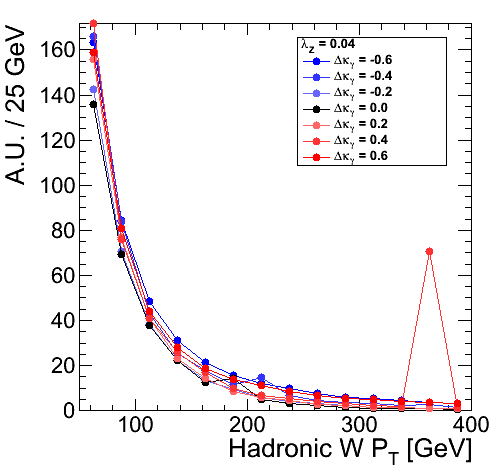
\includegraphics[width=0.48\textwidth]{figs/HadronicWpT_004.png}
%%    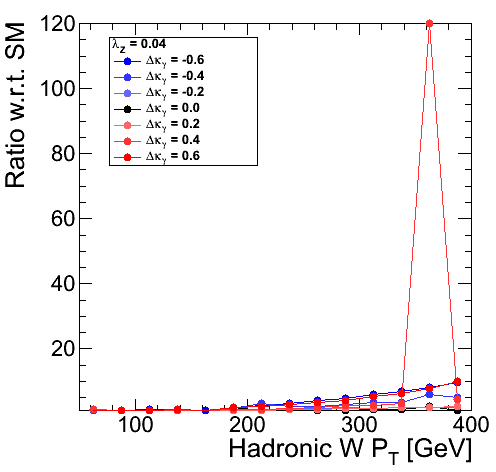
\includegraphics[width=0.48\textwidth]{figs/HadronicWpT_004_ratio.png}
    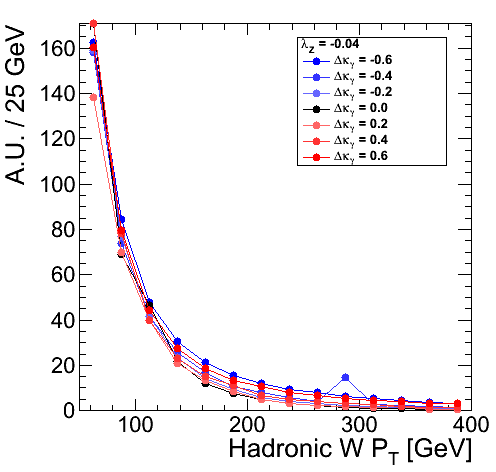
\includegraphics[width=0.48\textwidth]{figs/HadronicWpT_m004.png}
    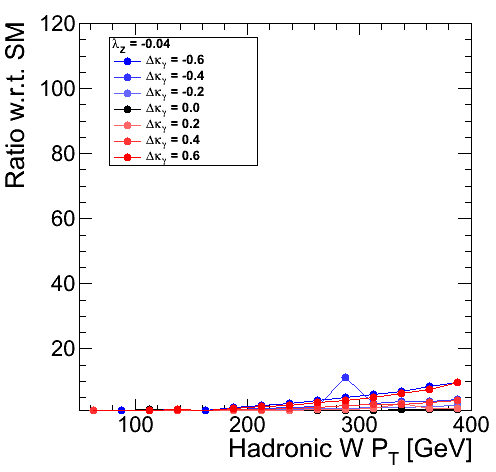
\includegraphics[width=0.48\textwidth]{figs/HadronicWpT_m004_ratio.png}
   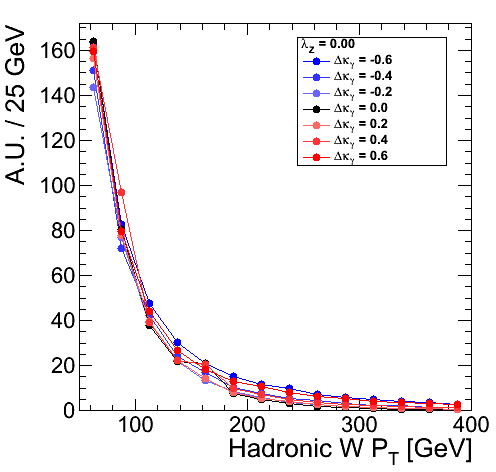
\includegraphics[width=0.48\textwidth]{figs/HadronicWpT_000.png}
    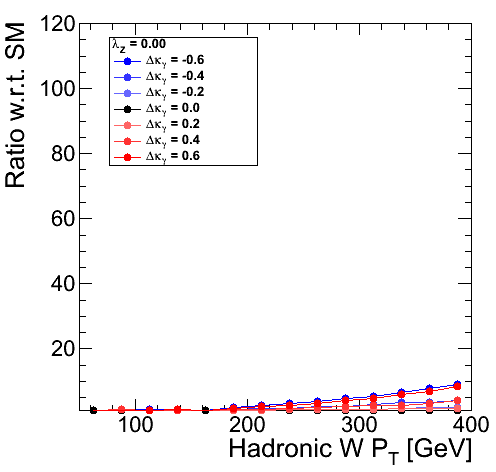
\includegraphics[width=0.48\textwidth]{figs/HadronicWpT_000_ratio.png}
    \caption{Dijet $p_T$ distribution (left) and its ratio relative to 
    the standard model coupling (right) for $\lambda_Z = 0.04$ (top row) and 
    $\lambda_Z = 0.00$ (bottom row)
    and various choices of $\Delta{\kappa_\gamma}$.}
%%    \caption{Dijet $p_T$ distribution (left) and its ratio relative to 
%%    the standard model coupling (right) for $\lambda_Z = \pm 0.04$ and various choices of $\Delta{\kappa_\gamma}$.}
    \label{fig:ww_dijetPt_atgcRatio004}}
\end{figure}
%%%%%%%%%%%%%%%%%%%%%%%%%%%%
%%%%%%%%%%%%%%%%%%%%%%%%%%%%
%%\begin{figure}[h!t]
%%  {\centering
%%    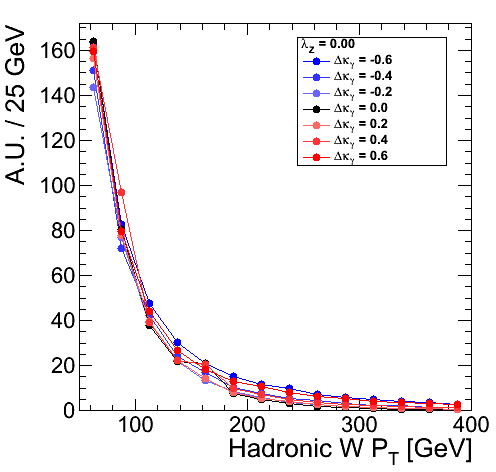
\includegraphics[width=0.48\textwidth]{figs/HadronicWpT_000.png}
%%    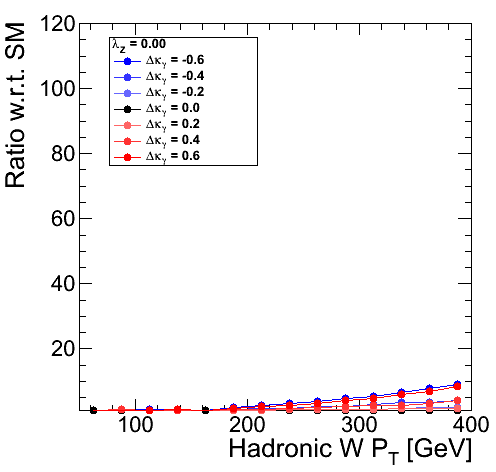
\includegraphics[width=0.48\textwidth]{figs/HadronicWpT_000_ratio.png}
%%    \caption{Dijet $p_T$ distribution (left) and its ratio relative to 
%%    the standard model coupling (right) for $\lambda_Z = 0.00$ and various choices of $\Delta{\kappa_\gamma}$.}
%%    \label{fig:ww_dijetPt_atgcRatio000}}
%%\end{figure}
%%%%%%%%%%%%%%%%%%%%%%%%%%%%
%\begin{figure}[h!t]
%  {\centering
%    \includegraphics[width=0.48\textwidth]{figs/atgcRatio_m06.png}
%    \includegraphics[width=0.48\textwidth]{figs/atgcRatio_06.png}
%    \caption{Ratio of the dijet $p_T$ distribution relative to 
%    the standard model coupling for $\lambda_Z = \pm 0.6$ and various choices of $\Delta{\kappa_\gamma}$.
%    }
%    \label{fig:ww_dijetPt_atgcRatio06}}
%\end{figure}
%%%%%%%%%%%%%%%%%%%%%%%%%%%%%
%%%%%%%%%%%%%%%%%%%%%%%%%%%%
%\begin{figure}[h!t]
%  {\centering
%    \includegraphics[width=0.48\textwidth]{figs/atgcRatio_m04.png}
%    \includegraphics[width=0.48\textwidth]{figs/atgcRatio_04.png}
%    \caption{Ratio of the dijet $p_T$ distribution relative to 
%    the standard model coupling for $\lambda_Z = \pm 0.4$ and various choices of $\Delta{\kappa_\gamma}$.
%    }
%    \label{fig:ww_dijetPt_atgcRatio04}}
%\end{figure}
%
%%%%%%%%%%%%%%%%%%%%%%%%%%%%
%%%%%%%%%%%%%%%%%%%%%%%%%%%%%
%\begin{figure}[h!t]
%  {\centering
%    \includegraphics[width=0.48\textwidth]{figs/atgcRatio_m02.png}
%    \includegraphics[width=0.48\textwidth]{figs/atgcRatio_02.png}
%    \caption{Ratio of the dijet $p_T$ distribution relative to 
%    the standard model coupling for $\lambda_Z = \pm 0.2$ and various choices of $\Delta{\kappa_\gamma}$.
%    }
%    \label{fig:ww_dijetPt_atgcRatio02}}
%\end{figure}
%%%%%%%%%%%%%%%%%%%%%%%%%%%%%
%
%%%%%%%%%%%%%%%%%%%%%%%%%%%%
The differential cross section as a function of the 
$p_T$ of either W boson can directly probe the anomalous couplings,
particularly at high $p_T$.
We use the the dijet $p_T$ distribution as an observable to set limit on 
anomalous couplings.
The dependence of the distribution on specific anomalous couplings 
is modeled by re-weighting the Pythia SM WW MC to the predictions 
of the MCFM~\cite{MCFM} NLO generator at the matrix-element level. 
The dijet $p_T$ distribution is found
to be consistent between the LO Pythia WW and the generator level LO 
MCFM without anomalous couplings, as can be seen in 
Figure~\ref{fig:ww_dijetPt_PythiaMCFM_comparison}. 
%%Therefore, anomalous coupling samples produced in MCFM can 
%%be used directly for the present study.
The anomalous coupling samples were produced with the values listed in 
Tables~\ref{tab:aTGC_generatedPoints}--\ref{tab:aTGC_generatedPoints2}.
Figure~\ref{fig:ww_dijetPt_PythiaMCFM_comparison}b shows the change in 
relative cross section compared to the standard model couplings 
as a function of anomalous coupling parameters.
Figures~\ref{fig:ww_dijetPt_atgcRatio06}--\ref{fig:ww_dijetPt_atgcRatio004} 
show the ratio of the dijet $p_T$ cross section relative to values for 
the standard model couplings for various choices of $\lambda_Z$ and 
$\Delta{\kappa_\gamma}$.
%%%%%%%%%%%%%%%%%%%%%%%%%%%%%
\begin{table}[h]
\begin{center}
  \begin{tabular}{l l c | l l c}
    \hline  \hline
    $\lambda_Z$  &  $\Delta{\kappa_\gamma}$  & Cross section ratio: $\sigma/\sigma_{SM}$ & 
    $\lambda_Z$  &  $\Delta{\kappa_\gamma}$  & Cross section ratio: $\sigma/\sigma_{SM}$\\\hline
-0.60 & 0.60 & 2.2794 $\pm$ 0.0021 & -0.60 & -0.60 & 2.3057 $\pm$ 0.0021 \\ 
      & 0.40 & 2.2308 $\pm$ 0.0021 &       & -0.40 & 2.2496 $\pm$ 0.0021 \\ 
      & 0.20 & 2.2041 $\pm$ 0.0022 &       & -0.20 & 2.2133 $\pm$ 0.0021 \\ 
      & 0.00 & 2.1985 $\pm$ 0.0021 & &     &                            \\ \hline
-0.40 & 0.60 & 1.5914 $\pm$ 0.0015 & -0.40 & -0.60 & 1.6206 $\pm$ 0.0015 \\ 
      & 0.40 & 1.5437 $\pm$ 0.0015 &       & -0.40 & 1.5641 $\pm$ 0.0017 \\ 
      & 0.20 & 1.5182 $\pm$ 0.0015 &       & -0.20 & 1.5268 $\pm$ 0.0016 \\ 
      & 0.00 & 1.5118 $\pm$ 0.0015 &       &       &                     \\ \hline
-0.36 & 0.60 & 1.5914 $\pm$ 0.0015 & -0.36 & -0.60 & 1.6206 $\pm$ 0.0015 \\ 
      & 0.40 & 1.5437 $\pm$ 0.0015 &       & -0.40 & 1.5641 $\pm$ 0.0017 \\ 
      & 0.20 & 1.5182 $\pm$ 0.0015 &       & -0.20 & 1.5268 $\pm$ 0.0016 \\ 
      & 0.00 & 1.5118 $\pm$ 0.0015 &       &       &                     \\ \hline
-0.32 & 0.60 & 1.5118 $\pm$ 0.0015 & -0.32 & -0.60 & 1.5268 $\pm$ 0.0016 \\ 
      & 0.40 & 1.5118 $\pm$ 0.0015 &       & -0.40 & 1.5268 $\pm$ 0.0016 \\ 
      & 0.20 & 1.5118 $\pm$ 0.0015 &       & -0.20 & 1.5268 $\pm$ 0.0016 \\ 
      & 0.00 & 1.5118 $\pm$ 0.0015 &       &       &                      \\ \hline
-0.28 & 0.60 & 1.5118 $\pm$ 0.0015 & -0.28 & -0.60 & 1.5268 $\pm$ 0.0016 \\ 
      & 0.40 & 1.5118 $\pm$ 0.0015 &       & -0.40 & 1.5268 $\pm$ 0.0016 \\ 
      & 0.20 & 1.5118 $\pm$ 0.0015 &       & -0.20 & 1.5268 $\pm$ 0.0016 \\ 
      & 0.00 & 1.5118 $\pm$ 0.0015 &       &       &                     \\ \hline
-0.24 & 0.60 & 1.1925 $\pm$ 0.0012 & -0.24 & -0.60 & 1.2235 $\pm$ 0.0012 \\ 
      & 0.40 & 1.1446 $\pm$ 0.0012 &       & -0.40 & 1.1662 $\pm$ 0.0012 \\ 
      & 0.20 & 1.1194 $\pm$ 0.0012 &       & -0.20 & 1.1293 $\pm$ 0.0011 \\ 
      & 0.00 & 1.1138 $\pm$ 0.0012 &       &       &                     \\ \hline
-0.20 & 0.60 & 1.1925 $\pm$ 0.0012 & -0.20 & -0.60 & 1.2235 $\pm$ 0.0012 \\ 
      & 0.40 & 1.1446 $\pm$ 0.0012 &       & -0.40 & 1.1662 $\pm$ 0.0012 \\ 
      & 0.20 & 1.1194 $\pm$ 0.0012 &       & -0.20 & 1.1293 $\pm$ 0.0011 \\ 
      & 0.00 & 1.1138 $\pm$ 0.0012 &       &       &                     \\ \hline
-0.16 & 0.60 & 1.1925 $\pm$ 0.0012 & -0.16 & -0.60 & 1.2235 $\pm$ 0.0012 \\ 
      & 0.40 & 1.1446 $\pm$ 0.0012 &       & -0.40 & 1.1662 $\pm$ 0.0012 \\ 
      & 0.20 & 1.1194 $\pm$ 0.0012 &       & -0.20 & 1.1293 $\pm$ 0.0011 \\ 
      & 0.00 & 1.1138 $\pm$ 0.0012 &       &       &                     \\ \hline
-0.12 & 0.60 & 1.1138 $\pm$ 0.0012 & -0.12 & -0.60 & 1.1293 $\pm$ 0.0011 \\ 
      & 0.40 & 1.1138 $\pm$ 0.0012 &       & -0.40 & 1.1293 $\pm$ 0.0011 \\
      & 0.20 & 1.1138 $\pm$ 0.0012 &       & -0.20 & 1.1293 $\pm$ 0.0011 \\ 
      & 0.00 & 1.1138 $\pm$ 0.0012 &       &       &                      \\ \hline
-0.08 & 0.60 & 1.1138 $\pm$ 0.0012 & -0.08 & -0.60 & 1.1293 $\pm$ 0.0011 \\ 
      & 0.40 & 1.1138 $\pm$ 0.0012 &       & -0.40 & 1.1293 $\pm$ 0.0011 \\ 
      & 0.20 & 1.1138 $\pm$ 0.0012 &       & -0.20 & 1.1293 $\pm$ 0.0011 \\ 
      & 0.00 & 1.1138 $\pm$ 0.0012 &       &       &                      \\ \hline
-0.04 & 0.60 & 1.1138 $\pm$ 0.0012 & -0.04 & -0.60 & 1.1293 $\pm$ 0.0011 \\ 
      & 0.40 & 1.1138 $\pm$ 0.0012 &       & -0.40 & 1.1293 $\pm$ 0.0011 \\ 
      & 0.20 & 1.1138 $\pm$ 0.0012 &       & -0.20 & 1.1293 $\pm$ 0.0011 \\ 
      & 0.00 & 1.1138 $\pm$ 0.0012 &       &       &                      \\ \hline
 0.00 & 0.60 & 1.1138 $\pm$ 0.0012 &  0.00 & -0.60 & 1.1293 $\pm$ 0.0011 \\ 
      & 0.40 & 1.1138 $\pm$ 0.0012 &       & -0.40 & 1.1293 $\pm$ 0.0011 \\ 
      & 0.20 & 1.1138 $\pm$ 0.0012 &       & -0.20 & 1.1293 $\pm$ 0.0011 \\ \hline
    \hline  
\end{tabular}
%%%%%%
\end{center}
\caption{\label{tab:aTGC_generatedPoints}
The anomalous coupling values for which the MCFM samples were generated and the corresponding 
change in cross section.}
\end{table}
%%%%%%%%%%%%%%%%%%%%%%%%%%%%%
%%%%%%%%%%%%%%%%%%%%%%%%%%%%%
\begin{table}[h]
\begin{center}
  \begin{tabular}{l l c | l l c}
    \hline  \hline
    $\lambda_Z$  &  $\Delta{\kappa_\gamma}$  & Cross section ratio: $\sigma/\sigma_{SM}$ & 
    $\lambda_Z$  &  $\Delta{\kappa_\gamma}$  & Cross section ratio: $\sigma/\sigma_{SM}$\\\hline
0.04 & 0.60 & 1.0785 $\pm$ 0.0013 & 0.04 & -0.60 & 1.1118 $\pm$ 0.0014 \\ 
     & 0.40 & 1.0315 $\pm$ 0.0020 &      & -0.40 & 1.0532 $\pm$ 0.0017 \\ 
     & 0.20 & 1.0063 $\pm$ 0.0014 &      & -0.20 & 1.0170 $\pm$ 0.0016 \\ 
     & 0.00 & 1.0000 $\pm$ 0.0015 &      &       &                      \\ \hline
0.08 & 0.60 & 1.0000 $\pm$ 0.0015 & 0.08 & -0.60 & 1.0170 $\pm$ 0.0016 \\ 
     & 0.40 & 1.0000 $\pm$ 0.0015 &      & -0.40 & 1.0170 $\pm$ 0.0016 \\ 
     & 0.20 & 1.0000 $\pm$ 0.0015 &      & -0.20 & 1.0170 $\pm$ 0.0016 \\ 
     & 0.00 & 1.0000 $\pm$ 0.0015 &      &       &                     \\ \hline
0.12 & 0.60 & 1.0000 $\pm$ 0.0015 & 0.12 & -0.60 & 1.0170 $\pm$ 0.0016 \\ 
     & 0.40 & 1.0000 $\pm$ 0.0015 &      & -0.40 & 1.0170 $\pm$ 0.0016 \\ 
     & 0.20 & 1.0000 $\pm$ 0.0015 &      & -0.20 & 1.0170 $\pm$ 0.0016 \\ 
     & 0.00 & 1.0000 $\pm$ 0.0015 &      &       &                     \\ \hline
0.16 & 0.60 & 1.2494 $\pm$ 0.0013 & 0.16 & -0.60 & 1.2864 $\pm$ 0.0013 \\ 
     & 0.40 & 1.2039 $\pm$ 0.0012 &      & -0.40 & 1.2276 $\pm$ 0.0012 \\ 
     & 0.20 & 1.1787 $\pm$ 0.0012 &      & -0.20 & 1.1905 $\pm$ 0.0012 \\ 
     & 0.00 & 1.1748 $\pm$ 0.0013 &      &       &                     \\ \hline
0.20 & 0.60 & 1.2494 $\pm$ 0.0013 & 0.20 & -0.60 & 1.2864 $\pm$ 0.0013 \\ 
     & 0.40 & 1.2039 $\pm$ 0.0012 &      & -0.40 & 1.2276 $\pm$ 0.0012 \\ 
     & 0.20 & 1.1787 $\pm$ 0.0012 &      & -0.20 & 1.1905 $\pm$ 0.0012 \\ 
     & 0.00 & 1.1748 $\pm$ 0.0013 &      &       &                     \\ \hline
0.24 & 0.60 & 1.2494 $\pm$ 0.0013 & 0.24 & -0.60 & 1.2864 $\pm$ 0.0013 \\ 
     & 0.40 & 1.2039 $\pm$ 0.0012 &      & -0.40 & 1.2276 $\pm$ 0.0012 \\ 
     & 0.20 & 1.1787 $\pm$ 0.0012 &      & -0.20 & 1.1905 $\pm$ 0.0012 \\ 
     & 0.00 & 1.1748 $\pm$ 0.0013 &      &       &                     \\ \hline
0.28 & 0.60 & 1.1748 $\pm$ 0.0013 & 0.28 & -0.60 & 1.1905 $\pm$ 0.0012 \\ 
     & 0.40 & 1.1748 $\pm$ 0.0013 &      & -0.40 & 1.1905 $\pm$ 0.0012 \\ 
     & 0.20 & 1.1748 $\pm$ 0.0013 &      & -0.20 & 1.1905 $\pm$ 0.0012 \\ 
     & 0.00 & 1.1748 $\pm$ 0.0013 &      &       &                     \\ \hline
0.32 & 0.60 & 1.1748 $\pm$ 0.0013 & 0.32 & -0.60 & 1.1905 $\pm$ 0.0012 \\ 
     & 0.40 & 1.1748 $\pm$ 0.0013 &      & -0.40 & 1.1905 $\pm$ 0.0012 \\ 
     & 0.20 & 1.1748 $\pm$ 0.0013 &      & -0.20 & 1.1905 $\pm$ 0.0012 \\ 
     & 0.00 & 1.1748 $\pm$ 0.0013 &      &       &                     \\ \hline
0.36 & 0.60 & 1.7073 $\pm$ 0.0016 & 0.36 & -0.60 & 1.7464 $\pm$ 0.0017 \\ 
     & 0.40 & 1.6615 $\pm$ 0.0018 &      & -0.40 & 1.6878 $\pm$ 0.0016 \\ 
     & 0.20 & 1.6382 $\pm$ 0.0016 &      & -0.20 & 1.6501 $\pm$ 0.0015 \\ 
     & 0.00 & 1.6330 $\pm$ 0.0016 &      &       &                     \\ \hline
0.40 & 0.60 & 1.7073 $\pm$ 0.0016 & 0.40 & -0.60 & 1.7464 $\pm$ 0.0017 \\ 
     & 0.40 & 1.6615 $\pm$ 0.0018 &      & -0.40 & 1.6878 $\pm$ 0.0016 \\ 
     & 0.20 & 1.6382 $\pm$ 0.0016 &      & -0.20 & 1.6501 $\pm$ 0.0015 \\ 
     & 0.00 & 1.6330 $\pm$ 0.0016 &      &       &                     \\ \hline  
0.60 & 0.60 & 2.4539 $\pm$ 0.0022 & 0.60 & -0.60 & 2.4935 $\pm$ 0.0023 \\ 
     & 0.40 & 2.4076 $\pm$ 0.0022 &      & -0.40 & 2.4356 $\pm$ 0.0022 \\ 
     & 0.20 & 2.3813 $\pm$ 0.0022 &      & -0.20 & 2.3967 $\pm$ 0.0022 \\ 
     & 0.00 & 2.3790 $\pm$ 0.0023 &      &                            \\ \hline  
    \hline  
\end{tabular}
%%%%%%
\end{center}
\caption{\label{tab:aTGC_generatedPoints2}
The anomalous coupling values for which the MCFM samples were generated and the corresponding 
change in cross section.}
\end{table}
%%%%%%%%%%%%%%%%%%%%%%%%%%%%%
%%%%%%%%%%%%%%%%%%%%%%%%%%%%
%%%%%%%%%%%%%%%%%%%%%%%%%%%%
%%%%%%%%%%%%%%%%%%%%%%%%%%%%
\subsection{Limit setting}
\label{sec:limits}
We use the dijet $p_T$ distribution as observable to set limit on anomalous couplings. 
We plot the dijet $p_T$ distribution in data and various standard model 
components using the event selection criteria described in section~\ref{sec:reco},
additionally requiring a dijet invariant mass selection of $75 < m_{jj} < 95$~\GeV,
in Fig.~\ref{fig:ww_dijetPt_stacked}. 
The figure also shows a typical anomalous coupling corresponding to 
$\lambda_Z = 0.2, \Delta{\kappa_\gamma} = 0.0$ for comparison.
%%%%%%%%%%%%%%%%%%%%%%%%%%%%
\begin{figure}[h!t]
  {\centering
    \includegraphics[width=0.48\textwidth]{figs/mu_noBtag_dijetPt.png}
    \includegraphics[width=0.48\textwidth]{figs/mu_btag_dijetPt.png}
    \includegraphics[width=0.48\textwidth]{figs/el_noBtag_dijetPt.png}
    \includegraphics[width=0.48\textwidth]{figs/el_btag_dijetPt.png}
    \caption{Comparison of the dijet $p_T$ distribution using the event 
    selection criteria described in section~\ref{sec:reco}, and with the requirement
    $75 < m_{jj} < 95$~\GeV : 
    muon no b-tag (upper left), muon b-tag (upper right), electron 
    no b-tag (lower left), electron b-tag (lower right).
    The individual components are normalized according to the fit 
    results of section~\ref{sec:mjj_fit} and corrected for the 
    dijet $p_T$ range being plotted.
    }
    \label{fig:ww_dijetPt_stacked}}
\end{figure}
%%%%%%%%%%%%%%%%%%%%%%%%%%%%
%%%%%%%%%%%%%%%%%%%%%%%%%%%%%


We use the ``Higgs Combination'' package \cite{cite:combine} for
setting exclusion limits. This package is a
RooStats\cite{cite:roostats}-based statistical analysis tool-set
recommended by the CMS Higgs PAG and approved by CMS statistics committee.

We take as inputs the dijet $p_T$
distributions for each signal model (\textit{i.e.},  
various choices of $\lambda_Z$ and $\Delta{\kappa_\gamma}$), 
data, and total background that
survive after analysis cuts. 
All of these distributions are segregated by lepton flavor and jet content,
which represent independent
channel inputs to the limit setter. 
We supply
these distributions over the range $50-400~\gev$ in the form of
histograms to the limit setter.


The limit setter is then set to utilize the ``asymptotic CL$_{s}$''
\cite{cite:asympcls1,cite:asympcls2} method. The resulting observed limit, as well as
the median expected limit and 1- and 2-sigma error bands, are plotted.
 %%%%%%%%%%%%%%%%%%%%%%%%%%%%%%
%%%%%%%%%%%%%%%%%%%%%%%%%%%%%%
%%%%%%%%%%%%%%%%%%%%%%%%%%%%%%
%%%%%%%%%%%%%%%%%%%%%%%%%%%%%%
\subsection{Systematic uncertainties considered for limit settings}
We considered the following sources of systematics.
%%%%%%%%%%%%%%%%%%%%%%%%%%%%%%%%%%%%%%%%%%%%
\subsubsection{Normalization of the standard model processes}
The uncertainty in the normalization of the sum of the standard model backgrounds 
(diboson, W+jets, $\ttbar$,  single top, QCD multi-jets, and Z+jets processes) 
is taken directly from the diboson signal extraction fit, as 
documented in section~\ref{sec:syst}.
%%%%%
\subsubsection{Normalization of the aTGC cross section}
Since we model the aTGC process via a differential ratio 
(in dijet $p_T$) relative to the standard model process, 
the cross section uncertainty is already accounted for in 
the normalization of the background. 
%%%%%%%%%%%%%%%%%%%%%%%%%%%%
\subsubsection{Luminosity uncertainty}
The latest recommendation for the uncertainty on LHC luminosity is 2.2$\%$~\cite{lumiPAS}.
We propagate LHC luminosity uncertainty of 2.2$\%$~\cite{lumiPAS} 
to the expected yield of the aTGC signal.
%%%%%%%%%%%%%%%%%%%%%%%%%%%%
\subsubsection{Lepton selection and trigger efficiency}
Systematic uncertainties in the trigger efficiencies in
Section~\ref{sec:trigger} are of the order of 1\%. Systematic
uncertainties in the lepton reconstruction and identification
efficiency scale factors are of the order of 2\%. 
%%%%%%%%%%%%%%%%%%%%%%%%%%%%
\subsubsection{Background shape uncertainty}
 The shape uncertainty of the W+jets background 
constitutes a systematic uncertainty. The alternative 
W+jets samples described in Sections~\ref{sec:wjetsShape}-\ref{sec:mjj_fit} 
do not have decent statistics in the tail of high dijet $p_T$ regime. 
Therefore, we take the variation in factorization/renormalization scale 
from MCFM LO. 
Using the same scale choice as used in our default MadGraph sample 
($q_0^2 = M_W^2 + p_{T, W}^2$), we generated samples with 
$q= 2~q_0$ and $q= 0.5~q_0$. 
We then take the maximal variation in the dijet $p_T$ shape with respect 
to the $q= q_0$ as a systematic uncertainty. 
The dijet $p_T$ spectrum has statistically insignificant variation 
when one includes background events with higher jet multiplicity 
(\textit{i. e.}, $\text{N}_{\text{jets}} >2$). 
Figure~\ref{fig:ww_dijetPt_stacked} shows the combined effect of this 
shape systematics.
%%%%%%%%%%%%%%%%%%%%%%%%%%%%
\subsubsection{Signal shape uncertainty}
Since the signal shape is derived from the 
NLO generator at the matrix-element level, the effect of 
factorization/renormalization scale is minuscule.
We verify this for a few aTGC points and assume 
this systematics to be negligible.
%%%%%%%%%%%%%%%%%%%%%%%%%%%%%%
%%%%%%%%%%%%%%%%%%%%%%%%%%%%%%
%%%%%%%%%%%%%%%%%%%%%%%%%%%%%%
%%%%%%%%%%%%%%%%%%%%%%%%%%%%%%
%% \subsection{Cut \& count limit using full \texorpdfstring{5.0 fb${}^{-1}$}{5.0/fb} data sample}
%% In Fig.~\ref{fig:FigLimitsFullData}a we show observed and expected values of the
%% CL${}_{S}$ statistic for anomalous coupling signals described above.
%% Exclusion limits in 2-dimensional $\lambda_Z:\Delta{\kappa_\gamma}$ plane
%% are computed at the 95\% confidence level (C.L.) by counting the events with  
%% dijet $pT > 200$~GeV (\textit{i. e.}, ``cut-and-count'' method). 
%% The 200~GeV threshold was chosen by optimizing the cut for expected limit.


%% We obtain the following exclusion limits\\

%% Expected: \\
%% \hspace*{6 mm} $ -0.105 < \, \, \lambda_Z \, \, < 0.101$  \, \, \,(assuming $\Delta{\kappa_\gamma}=0$)\\ 
%% \hspace*{6 mm} $ -0.396 < \, \, \Delta{\kappa_\gamma} \, \, < 0.450$  \, \, \,(assuming $\lambda_Z=0$)\\

%% Observed: \\ 
%% \hspace*{6 mm} $ -0.092 < \, \, \lambda_Z \, \, < 0.072$  \, \, \, (assuming $\Delta{\kappa_\gamma}=0$) \\
%% \hspace*{6 mm} $ -0.312 < \, \, \Delta{\kappa_\gamma} \, \, < 0.358$  \, \, \, (assuming $\lambda_Z=0$).
%% %%%%%%%%%%%%%%%%%%%
%% %%%%%%%%%%%%%%%%%%%
%% \begin{figure}[bthp]
%%   {\centering
%% \includegraphics[width=0.48\textwidth]{figs/atgc_limits_noshape_contours_dijetptmin200gev.png}
%% %%\includegraphics[width=0.45\textwidth]{figs/limitLambdaZ.pdf}
%% %%\includegraphics[width=0.45\textwidth]{figs/limitDkappaGamma.pdf}
%% \caption{
%% Limits on 
%% anomalous triple gauge couplings in $\lambda_Z:\Delta{\kappa_\gamma}$ plane obtained using 
%% cut and count method.
%% %%: (a) as 2-dimensional contour in 
%% %%$\lambda_Z:\Delta{\kappa_\gamma}$ plane, (b) in $\lambda_Z$, and 
%% %%(c) in $\Delta{\kappa_\gamma}$.
%% }
%% \label{fig:FigLimitsFullData}}
%% }
%% \end{figure}
%%%%%%%%%%%%%%%%%%%


%%%%%%%%%%%%%%%%%%%%%%%%%%%%%%
\subsection{Shape-based limit using full \texorpdfstring{5.0 fb${}^{-1}$}{5.0/fb} data sample}
In Figures~\ref{fig:limitshape2d} and \ref{fig:limitshape1d} we present
shape-based exclusion limits using the full dijet $pT$ spectrum.  Exclusion
limits in 2-dimensional $\lambda_Z:\Delta{\kappa_\gamma}$ plane and individually
for $\lambda_Z$ and $\Delta{\kappa_\gamma}$ are computed at the 95\% C.L.

We obtain the following observed exclusion limits:

%% Expected: \\
%% \hspace*{6 mm} $ -0.100 < \, \, \lambda_Z \, \, < 0.086$  \, \, \,(assuming $\Delta{\kappa_\gamma}=0$)\\ 
%% \hspace*{6 mm} $ -0.315 < \, \, \Delta{\kappa_\gamma} \, \, < 0.349$  \, \, \,(assuming $\lambda_Z=0$)\\

%% Observed: \\ 
\hspace*{6 mm} $ -0.038 < \, \, \lambda_Z \, \, < 0.03$  \, \, \, (assuming $\Delta{\kappa_\gamma}=0$) \\
\hspace*{6 mm} $ -0.11 < \, \, \Delta{\kappa_\gamma} \, \, < 0.14$  \, \, \, (assuming $\lambda_Z=0$).

These limits are consistent with the SM prediction. 
%%%%%%%%%%%%%%%%%%%
%%%%%%%%%%%%%%%%%%%
\begin{figure}[bthp]
\includegraphics[width=0.8\textwidth]{figs/lz_dkg_2dlimit.pdf}
%% \includegraphics[width=0.48\textwidth]{figs/atgc_limits_withshape_nosyst.png}
\caption{\label{fig:limitshape2d}
The observed and expected values of the shape-based  CL${}_{\textrm{S}}$ limit for 
anomalous triple gauge couplings in $\lambda_Z:\Delta{\kappa_\gamma}$ plane.
}
\end{figure}
\begin{figure}[bthp]
\includegraphics[width=0.48\textwidth]{figs/lz_1dlimit.pdf}
\includegraphics[width=0.48\textwidth]{figs/dkg_1dlimit.pdf}
\caption{\label{fig:limitshape1d}
The observed and expected values of the shape-based  CL${}_{\textrm{S}}$ limit for 
anomalous triple gauge couplings in $\lambda_Z$ (left) and $\Delta{\kappa_\gamma}$ (right)
including all systematic uncertainties.
}
\end{figure}
%%%%%%%%%%%%%%%%%%%


%%%%%%%%%%%%%%%%%%%%%%%%%%%%%%
\subsection{Shape-based limit using non b-tag categories only}
At the 95\% confidence level (CL) 
we obtain the following 1-dimensional observed upper limits 
assuming the SM value for the other parameter: 
$ -0.038 < \lambda_Z < 0.030$, 
$ -0.111 < \Delta{\kappa_\gamma} < 0.142$.

%%%%%%%%%%%%%%%%%%%
%%%%%%%%%%%%%%%%%%%
\begin{figure}[bthp]
\includegraphics[width=0.8\textwidth]{figs/lz_dkg_2dlimit2ch.pdf}
\caption{\label{fig:limitshape2d2ch}
Non b-tag channels only: The observed and expected values of the shape-based  CL${}_{\textrm{S}}$ limit for 
anomalous triple gauge couplings in $\lambda_Z:\Delta{\kappa_\gamma}$ plane.
}
\end{figure}
\begin{figure}[bthp]
\includegraphics[width=0.48\textwidth]{figs/lz_1dlimit2ch.pdf}
\includegraphics[width=0.48\textwidth]{figs/dkg_1dlimit2ch.pdf}
\caption{\label{fig:limitshape1d2ch}
Non b-tag channels only: The observed and expected values of the shape-based  CL${}_{\textrm{S}}$ limit for 
anomalous triple gauge couplings in $\lambda_Z$ (left) and $\Delta{\kappa_\gamma}$ (right)
including all systematic uncertainties.
}
\end{figure}
%%%%%%%%%%%%%%%%%%%


\clearpage
